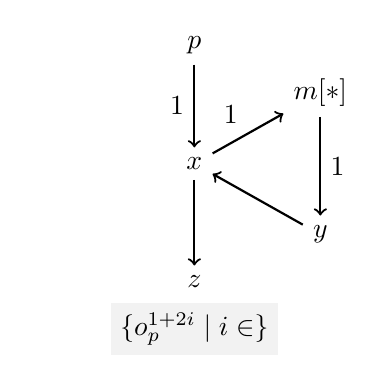
\begin{tikzpicture}[scale=1,thick]
    \node (p) at (0, 0) {$\textpurple{p}$};
    \node (x) at (0, -1.5) {$x$};
    \node (m) at (1.6, -0.6) {$m[*]$};
    \node (y) at (1.6, -2.4) {$y$};
    \node (z) at (0, -3) {$z$};
    \node[fill=gray!10] at (0, -3.6) {$\{o_p^{1 + 2i} \mid  i \in \nats\}$};

    \draw [->] (p) --node[left]{$1$} (x);
    \draw [->] (x) --node[above left]{$1$} (m);
    \draw [->] (m) --node[right]{$1$} (y);
    \draw [->] (y) -- (x);
    \draw [->] (x) -- (z);

    \node at (-2, 0) {};
\end{tikzpicture}
